\subsection{Conjuction finder}

GeospaceLAB provides a convenient method to find conjunctions between satellite trajectories and ground station locations. The Swarm \texttt{Dataset} has the built-in method \texttt{find\_conjunctions} to find conjunctions between the Swarm satellite and a station. The following function demonstrates how to use this method to find conjunctions between the Swarm A satellite and the EISCAT Tromsø site.

This method also check the data avaibility of the Swarm data product during the conjunction time, and only return the conjunctions with data available.

\begin{verbatim}
import datetime
import matplotlib.pyplot as plt
import numpy as np
import pathlib

import geospacelab.visualization.mpl.dashboards as dashboards
\end{verbatim}

\begin{verbatim}
dt_fr = datetime.datetime(2024, 5, 10, 0, )
dt_to = datetime.datetime(2024, 5, 13, 0, 0)

site_info = {
    'glat': 69.58, 'glon': 19.23, 'alt': 0. # EISCAT Tromso site
}

db = dashboards.TSDashboard(
    dt_fr=dt_fr, dt_to=dt_to, figure_config={'figsize': (8, 10)},
    timeline_extra_labels=['GEO_LAT', 'GEO_LON', 'APEX_LAT', 'APEX_LON', 'APEX_MLT',]
    )

ds_fac = db.dock(
    datasource_contents=['esa_eo', 'swarm', 'l2daily', 'fac_tms'], 
    product_version='latest', # 'latest' (default),
    sat_id='A', add_APEX=False)

conj_list = ds_fac.get_conjunction_with_site(
        glat_site=site_info['glat'], 
        glon_site=site_info['glon'], 
        alt_site=site_info['alt'],
        # Elevation limit for conjunctions. 
        # Only conjunctions with satellite elevation above 
        # the site higher than this limit 
        # will be included in the conjunction list.
        el_lim=60.,
        # Whether to print the conjunction list.
        print_conj_list=True,
    )
\end{verbatim}

\begin{verbatim}
Create a new figure: Figure(800x1000).
\end{verbatim}

\begin{verbatim}
Load IGRF coefficients ...
\end{verbatim}

\begin{verbatim}
Searching the data product "FAC_TMS" with the version "latest" on the server...
The file [PosixPath('/data/afys -ionosphere/data/ESA/SWARM/Level2daily/FAC_TMS/0401/Sat_A/2024/SW_OPER_FACATMS_2F_20240510T000000_20240510T235959_0401.cdf')] already exists: skip downloading.
The file [PosixPath('/data/afys -ionosphere/data/ESA/SWARM/Level2daily/FAC_TMS/0401/Sat_A/2024/SW_OPER_FACATMS_2F_20240511T000000_20240511T235959_0401.cdf')] already exists: skip downloading.
The file [PosixPath('/data/afys -ionosphere/data/ESA/SWARM/Level2daily/FAC_TMS/0401/Sat_A/2024/SW_OPER_FACATMS_2F_20240512T000000_20240512T235959_0401.cdf')] already exists: skip downloading.
The file [PosixPath('/data/afys -ionosphere/data/ESA/SWARM/Level2daily/FAC_TMS/0401/Sat_A/2024/SW_OPER_FACATMS_2F_20240513T000000_20240513T235959_0401.cdf')] already exists: skip downloading.
4 conjunction(s) found:
Index  Time (Start)         EL (Start) AZ (Start) D (Start)  Time (Highest)            EL (Highest)    AZ (Highest)    D (Highest)     Time (End)           EL (End)   AZ (End)   D (End)    Duration(s)
0      2024 -05 -10 06:32:18  60.34      232.93     246.36     2024 -05 -10 06:32:51       79.66           272.73          79.71           2024 -05 -10 06:33:24  60.20      329.70     247.55     66.00     
1      2024 -05 -10 17:41:29  60.04      287.70     249.06     2024 -05 -10 17:41:55       69.08           268.60          166.19          2024 -05 -10 17:42:21  60.19      245.18     247.71     52.00     
2      2024 -05 -11 06:03:25  60.43      119.23     245.44     2024 -05 -11 06:03:53       71.16           91.13           148.55          2024 -05 -11 06:04:20  60.45      69.68      245.11     55.00     
3      2024 -05 -11 17:12:23  60.56      20.83      243.93     2024 -05 -11 17:12:56       81.87           86.84           62.33           2024 -05 -11 17:13:30  60.28      133.15     246.84     67.00
\end{verbatim}

\begin{verbatim}
<FigureBase size 800x1000 with 0 Axes>
\end{verbatim}

The following function shows the time series plots with the conjunction with the EISCAT Tromsø site. The conjunction time is indicated by the vertical dashed line in the plot.

\begin{verbatim}
def test_conjunction_with_site():
    """Test Swarm EFI/LP 1B data product
    
    """
    dt_fr = datetime.datetime(2024, 5, 10, 0, )
    dt_to = datetime.datetime(2024, 5, 13, 0, 0)

    site_info = {
        'glat': 69.58, 'glon': 19.23, 'alt': 0. # EISCAT Tromso site
    }
    
    db = dashboards.TSDashboard(
        dt_fr=dt_fr, dt_to=dt_to, figure_config={'figsize': (8, 10)},
        timeline_extra_labels=['GEO_LAT', 'GEO_LON', 'APEX_LAT', 'APEX_LON', 'APEX_MLT',]
        )

    ds_fac = db.dock(
        datasource_contents=['esa_eo', 'swarm', 'l2daily', 'fac_tms'], 
        product_version='latest', # 'latest' (default),
        sat_id='A', add_APEX=False)
    
    conj_list = ds_fac.get_conjunction_with_site(
         glat_site=site_info['glat'], 
         glon_site=site_info['glon'], 
         alt_site=site_info['alt'],
         el_lim=60.,
         print_conj_list=True,
     )
    conj_data = conj_list[1]
    dt_fr_to_show = conj_data['DATETIME_0']
    dt_to_to_show = conj_data['DATETIME_1']
    
    ds_fac.dt_fr = dt_fr_to_show
    ds_fac.dt_to = dt_to_to_show
    ds_fac.time_filter_by_range()
    ds_fac.convert_to_APEX()
    
    ds_efi_lp = db.dock(
        dt_fr=dt_fr_to_show, dt_to=dt_to_to_show,
        datasource_contents=['esa_eo', 'swarm', 'l1b', 'efi_lp'], 
        product_version='latest', # 'latest' (default),
        sat_id='A', add_APEX=True)
    
    ds_mag_lr = db.dock(
        dt_fr=dt_fr_to_show, dt_to=dt_to_to_show,
        datasource_contents=['esa_eo', 'swarm', 'l1b', 'mag_lr'], 
        from_HAPI=True,
        product_version='latest', # 'latest' (default),
        sat_id='A', add_APEX=True)
    
    panel_layouts = [
        [ds_efi_lp['n_e']],
        [ds_efi_lp['n_i']],
        [ds_efi_lp['T_e']],
        [ds_mag_lr['B_res_Model_N'], ds_mag_lr['B_res_Model_E'], ds_mag_lr['B_res_Model_C']],
        [ds_fac['j_r']],
        [ds_fac['j_FA']],
    ]

    db.set_layout(panel_layouts=panel_layouts)
    db.draw(
        dt_fr=dt_fr_to_show, dt_to=dt_to_to_show,
    )
    
    # Add a vertical line to indicate the conjunction time
    db.add_vertical_line(
        conj_data['DATETIME'], label='EISCAT TRO', color='red', linestyle=' - -', linewidth=1.5,
    )
    db.add_title(title='Swarm -{} - EISCAT Tromso conjunction'.format(ds_fac.sat_id), fontsize='medium', append_time=True)

    return db
db = test_conjunction_with_site()
db.show()
\end{verbatim}

\begin{verbatim}
Create a new figure: Figure(800x1000).
Searching the data product "FAC_TMS" with the version "latest" on the server...
The file [PosixPath('/data/afys -ionosphere/data/ESA/SWARM/Level2daily/FAC_TMS/0401/Sat_A/2024/SW_OPER_FACATMS_2F_20240510T000000_20240510T235959_0401.cdf')] already exists: skip downloading.
The file [PosixPath('/data/afys -ionosphere/data/ESA/SWARM/Level2daily/FAC_TMS/0401/Sat_A/2024/SW_OPER_FACATMS_2F_20240511T000000_20240511T235959_0401.cdf')] already exists: skip downloading.
The file [PosixPath('/data/afys -ionosphere/data/ESA/SWARM/Level2daily/FAC_TMS/0401/Sat_A/2024/SW_OPER_FACATMS_2F_20240512T000000_20240512T235959_0401.cdf')] already exists: skip downloading.
The file [PosixPath('/data/afys -ionosphere/data/ESA/SWARM/Level2daily/FAC_TMS/0401/Sat_A/2024/SW_OPER_FACATMS_2F_20240513T000000_20240513T235959_0401.cdf')] already exists: skip downloading.
4 conjunction(s) found:
Index  Time (Start)         EL (Start) AZ (Start) D (Start)  Time (Highest)            EL (Highest)    AZ (Highest)    D (Highest)     Time (End)           EL (End)   AZ (End)   D (End)    Duration(s)
0      2024 -05 -10 06:32:18  60.34      232.93     246.36     2024 -05 -10 06:32:51       79.66           272.73          79.71           2024 -05 -10 06:33:24  60.20      329.70     247.55     66.00     
1      2024 -05 -10 17:41:29  60.04      287.70     249.06     2024 -05 -10 17:41:55       69.08           268.60          166.19          2024 -05 -10 17:42:21  60.19      245.18     247.71     52.00     
2      2024 -05 -11 06:03:25  60.43      119.23     245.44     2024 -05 -11 06:03:53       71.16           91.13           148.55          2024 -05 -11 06:04:20  60.45      69.68      245.11     55.00     
3      2024 -05 -11 17:12:23  60.56      20.83      243.93     2024 -05 -11 17:12:56       81.87           86.84           62.33           2024 -05 -11 17:13:30  60.28      133.15     246.84     67.00     
Searching the data product "EFI_LP" with the version "latest" on the server...
The file [PosixPath('/data/afys -ionosphere/data/ESA/SWARM/Level1b/EFI_LP/0701/Sat_A/2024/SW_OPER_EFIA_LP_1B_20240510T000000_20240510T235959_0701_MDR_EFI_LP.cdf')] already exists: skip downloading.
/opt/anaconda3/envs/Swarm/lib/python3.12/site -packages/numpy/_core/numeric.py:476: RuntimeWarning: invalid value encountered in cast
  multiarray.copyto(res, fill_value, casting='unsafe')
INFO: Loading data from HAPI for server https://vires.services/hapi, dataset SW_OPER_MAGA_LR_1B, parameters Timestamp,Latitude,Longitude,Radius.
INFO: Data loaded from HAPI.
INFO: Loading data from HAPI for server https://vires.services/hapi, dataset SW_OPER_MAGA_LR_1B, parameters F,dF_Sun,dF_AOCS,dF_other,F_error,B_VFM,B_NEC,dB_Sun,dB_AOCS,dB_other,B_error.
INFO: Data loaded from HAPI.
INFO: Loading data from HAPI for server https://vires.services/hapi, dataset SW_OPER_MAGA_LR_1B, parameters q_NEC_CRF,Att_error,Flags_F,Flags_B,Flags_q,Flags_Platform,ASM_Freq_Dev.
INFO: Data loaded from HAPI.
INFO: Loading data from HAPI for server https://vires.services/hapi, dataset SW_OPER_MAGA_LR_1B, parameters SyncStatus,B_NEC_Model,F_Model,F_res_Model,B_NEC_res_Model.
INFO: Data loaded from HAPI.
WARNING: Variable CDF_EPOCH is not in the default variable names and does not match the patterns for automatically assigning configured variable names. It will be added without a configured variable name, and may not be included in the default panels for plotting and analysis. Please check if this variable should be included in the default variable names or if it follows the naming patterns for automatic assignment of configured variable names.
WARNING: Variable SC_GEO_R is not in the default variable names and does not match the patterns for automatically assigning configured variable names. It will be added without a configured variable name, and may not be included in the default panels for plotting and analysis. Please check if this variable should be included in the default variable names or if it follows the naming patterns for automatic assignment of configured variable names.
WARNING: Variable B_NEC_Model is not in the default variable names and does not match the patterns for automatically assigning configured variable names. It will be added without a configured variable name, and may not be included in the default panels for plotting and analysis. Please check if this variable should be included in the default variable names or if it follows the naming patterns for automatic assignment of configured variable names.
WARNING: Variable B_NEC_res_Model is not in the default variable names and does not match the patterns for automatically assigning configured variable names. It will be added without a configured variable name, and may not be included in the default panels for plotting and analysis. Please check if this variable should be included in the default variable names or if it follows the naming patterns for automatic assignment of configured variable names.
/opt/anaconda3/envs/Swarm/lib/python3.12/site -packages/numpy/_core/numeric.py:476: RuntimeWarning: invalid value encountered in cast
  multiarray.copyto(res, fill_value, casting='unsafe')
WARNING: Negative values of error detected in GeospaceLab Variable object <name: j_r, value: array([[  3.08981391],
       [  2.98925703],
       [  1.56633446],
       [ -1.13820387],
       [  1.34360429],
       [  1.20251135],
       [ -1.2249717 ],
       [  3.12994392],
       [  0.40065637],
       [ -0.16233794],
       [  5.1499497 ],
       [  0.52370211],
       [ -1.09764934],
       [  6.07112128],
       [ -0.59552206],
       [ 14.15920087],
       [  0.95167483],
       [  1.0512454 ],
       [  2.59472964],
       [  2.24155043],
       [  0.10525129],
       [ -0.12611275],
       [  2.54786862],
       [  1.12647161],
       [  2.12356771],
       [  9.03824309],
       [ -6.44872064],
       [ 20.03705361],
       [ 19.53691737],
       [ 20.52376949],
       [ -0.89872449],
       [  3.19756193],
       [  5.11868821],
       [ -4.45562301],
       [  4.36727181],
       [  9.92268407],
       [ -13.69750467],
       [ -17.54984701],
       [  0.65148948],
       [ -0.40276721],
       [ -1.6018592 ],
       [ -1.06106664],
       [  0.08647688],
       [ -0.27753619],
       [ -0.37992582],
       [  0.17879571],
       [  0.75046254],
       [ -0.13289712],
       [ -0.90712415],
       [  0.91768621],
       [  0.75739485],
       [ -1.04945885]]), unit: muA/m^2>
\end{verbatim}

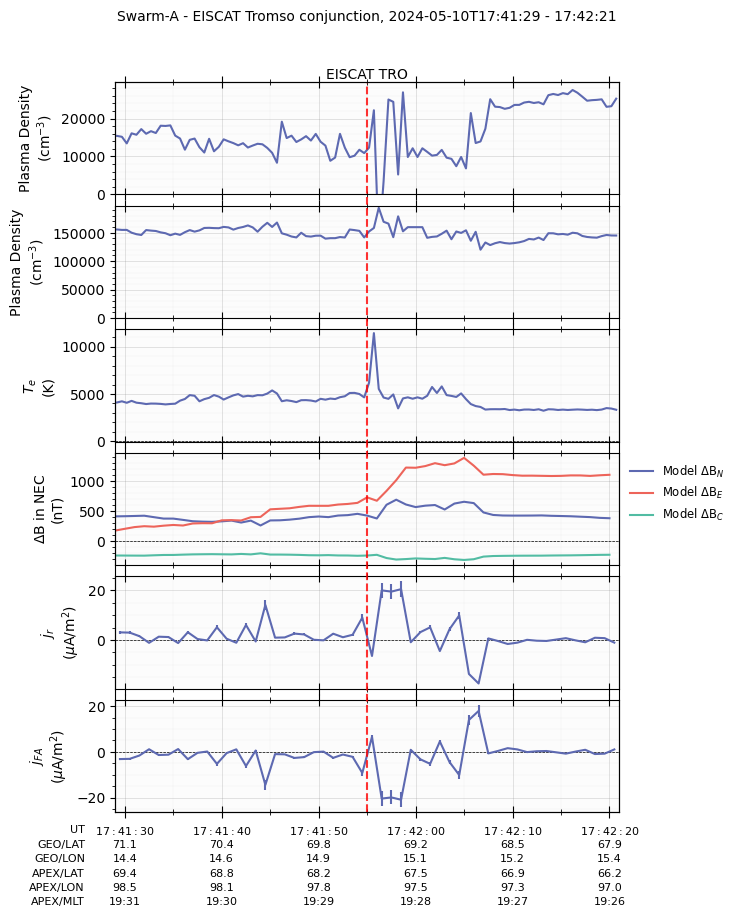
\includegraphics[width=0.7\linewidth]{files/f9eec9f1d29614cd6b8931443fa15605.png}